\documentclass{article}
\usepackage{amssymb,amsmath}
\usepackage{ifxetex,ifluatex}
\ifxetex
  \usepackage{fontspec,xltxtra,xunicode}
  \defaultfontfeatures{Mapping=tex-text,Scale=MatchLowercase}
\else
  \ifluatex
    \usepackage{fontspec}
    \defaultfontfeatures{Mapping=tex-text,Scale=MatchLowercase}
  \else
    \usepackage[utf8]{inputenc}
  \fi
\fi
\usepackage{ctable}
\usepackage{float} % provides the H option for float placement
\usepackage{graphicx}
% We will generate all images so they have a width \maxwidth. This means
% that they will get their normal width if they fit onto the page, but
% are scaled down if they would overflow the margins.
\makeatletter
\def\maxwidth{\ifdim\Gin@nat@width>\linewidth\linewidth
\else\Gin@nat@width\fi}
\makeatother
\let\Oldincludegraphics\includegraphics
\renewcommand{\includegraphics}[1]{\Oldincludegraphics[width=\maxwidth]{#1}}
\ifxetex
  \usepackage[setpagesize=false, % page size defined by xetex
              unicode=false, % unicode breaks when used with xetex
              xetex]{hyperref}
\else
  \usepackage[unicode=true]{hyperref}
\fi
\hypersetup{breaklinks=true, pdfborder={0 0 0}}
\setlength{\parindent}{0pt}
\setlength{\parskip}{6pt plus 2pt minus 1pt}
\setlength{\emergencystretch}{3em}  % prevent overfull lines
\setcounter{secnumdepth}{0}

\title{Crosstable}
\author{(Username not set) (E-mail address not set)}
\date{2011--04--26 20:25 CET}

\begin{document}
\maketitle

\subsection{Description}

Returning the Chi-squared test of two given variables with count,
percentages and Pearson's residuals table.

\subsubsection{Variable description}

Two variables specified: * ``gender'' (``Gender'') with 709 and *
``dwell'' (``Dwelling'') with 709 valid values.

\subsubsection{Counts}

\ctable[pos = H, center, botcap]{llll}
{% notes
}
{% rows
\FL
 & \textbf{city} & \textbf{small town} & \textbf{village}
\ML
male & 380 & 30 & 22
\\\noalign{\medskip}
female & 262 & 6 & 9
\LL
}

\subsubsection{Percentages}

\ctable[pos = H, center, botcap]{llll}
{% notes
}
{% rows
\FL
 & \textbf{city} & \textbf{small town} & \textbf{village}
\ML
male & 0.5360 & 0.0423 & 0.0310
\\\noalign{\medskip}
female & 0.3695 & 0.0085 & 0.0127
\LL
}

\paragraph{Row percentages}

\ctable[pos = H, center, botcap]{llll}
{% notes
}
{% rows
\FL
 & \textbf{city} & \textbf{small town} & \textbf{village}
\ML
male & 0.8796 & 0.0694 & 0.0509
\\\noalign{\medskip}
female & 0.9458 & 0.0217 & 0.0325
\LL
}

\paragraph{Column percentages}

\ctable[pos = H, center, botcap]{llll}
{% notes
}
{% rows
\FL
 & \textbf{city} & \textbf{small town} & \textbf{village}
\ML
male & 0.5919 & 0.8333 & 0.7097
\\\noalign{\medskip}
female & 0.4081 & 0.1667 & 0.2903
\LL
}

\subsubsection{Chi-squared test}

\ctable[pos = H, center, botcap]{llll}
{% notes
}
{% rows
\FL
 & \textbf{X-squared} & \textbf{df} & \textbf{p-value}
\ML
X-squared & 9.72 & 2.00 & 0.01
\LL
}

It seems that a real association can be pointed out between
\emph{gender} and \emph{dwell} by the \emph{Pearson's Chi-squared test}
(χ=9.7188 at the degree of freedom being 2) at the significance level of
0.0078. Based on Goodman and Kruskal's lambda it seems that \emph{dwell}
(λ=0.7581) has an effect on \emph{gender} (λ=0) if we assume both
variables to be nominal. The association between the two variables seems
to be weak based on Cramer's V (0.0828).

\paragraph{Pearson's residuals}

\ctable[pos = H, center, botcap]{llll}
{% notes
}
{% rows
\FL
 & \textbf{city} & \textbf{small town} & \textbf{village}
\ML
male & --2.9409 & 2.8277 & 1.1713
\\\noalign{\medskip}
female & 2.9409 & --2.8277 & --1.1713
\LL
}

\paragraph{Mosaic chart}

\begin{figure}[htbp]
\centering
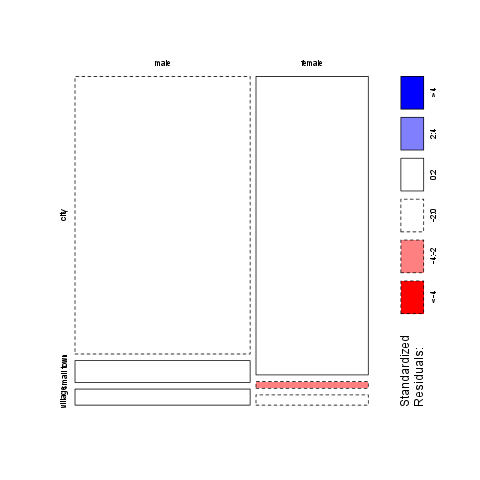
\includegraphics{66ba5aa603e08fec150848bb688f0953.png}
\caption{}
\end{figure}

\end{document}
